 \documentclass[10pt,twoside]{article}
\usepackage[ngerman]{babel}
\usepackage[utf8]{inputenc}
\usepackage{textcomp,gensymb}
\usepackage{longtable}
%\usepackage[latin1]{inputenc}
\usepackage{amsmath,thmtools}
\usepackage{array}
\usepackage{enumitem} 
\usepackage{amstext}
\usepackage{pdflscape}
\usepackage[separate-uncertainty]{siunitx}
\usepackage{amssymb}
\usepackage{stmaryrd}
\usepackage{tabularx}
\usepackage{verbatim}
\usepackage{mathrsfs}
\usepackage{extarrows}
\usepackage[arrow, matrix, curve]{xy}
\usepackage[centering,includeheadfoot,top=25mm, left=40mm, right=25mm, bottom=30mm]{geometry}
\usepackage{gensymb}
\usepackage{graphicx}
\usepackage{framed}
\usepackage[usenames,dvipsnames]{xcolor}
\usepackage{float}
\usepackage{graphicx} 
\usepackage{sidecap}
\usepackage{tikz,lipsum,lmodern}
\usepackage{import}
\usepackage{fancyhdr}
\usepackage{fancybox}
\usepackage{graphicx}
\usepackage{caption}
\usepackage{subcaption}
\usepackage{esint}
\parskip 10pt
\parindent 0pt
\DeclareGraphicsRule{.tif}{png}{.png}{`convert #1 `basename #1 .tif`.png} 
\makeindex
\usepackage[colorlinks,pdfpagelabels,pdfstartview = FitH,bookmarksopen = true,bookmarksnumbered = true,linkcolor = black,plainpages =false,hypertexnames = false,citecolor = black] {hyperref}
\makeatletter
\def\@tocline#1#2#3#4#5#6#7{\relax
  \ifnum #1>\c@tocdepth % then omit
  \else
    \par \addpenalty\@secpenalty\addvspace{#2}%
    \begingroup \hyphenpenalty\@M
    \@ifempty{#4}{%
      \@tempdima\csname r@tocindent\number#1\endcsname\relax
    }{%
      \@tempdima#4\relax
    }%
    \parindent\z@ \leftskip#3\relax \advance\leftskip\@tempdima\relax
    \rightskip\@pnumwidth plus4em \parfillskip-\@pnumwidth
    #5\leavevmode\hskip-\@tempdima
      \ifcase #1
       \or\or \hskip 1em \or \hskip 2em \else \hskip 3em \fi%
      #6\nobreak\relax
    \dotfill\hbox to\@pnumwidth{\@tocpagenum{#7}}\par
    \nobreak
    \endgroup
  \fi}
  \setcounter{tocdepth}{3}
\makeatother
%%%%%%%%%%%%%%%%%%%%%%%RedeclareMathOperator
\makeatletter
\newcommand\RedeclareMathOperator{%
  \@ifstar{\def\rmo@s{m}\rmo@redeclare}{\def\rmo@s{o}\rmo@redeclare}%
}
% this is taken from \renew@command
\newcommand\rmo@redeclare[2]{%
  \begingroup \escapechar\m@ne\xdef\@gtempa{{\string#1}}\endgroup
  \expandafter\@ifundefined\@gtempa
     {\@latex@error{\noexpand#1undefined}\@ehc}%
     \relax
  \expandafter\rmo@declmathop\rmo@s{#1}{#2}}
% This is just \@declmathop without \@ifdefinable
\newcommand\rmo@declmathop[3]{%
  \DeclareRobustCommand{#2}{\qopname\newmcodes@#1{#3}}%
}
\@onlypreamble\RedeclareMathOperator
\makeatother
\renewcommand{\sectionmark}[1]{\markboth{#1}{}}
\lhead{\fancyplain{}{\textit{\leftmark}}}
%%%%%%%%%%%%%%%%%%%%%%%%%%%%%%%%%%%%%%%%%%%%%%%%%%%%%%%%%%%%%%%%%%%%%%%%%%%%%%%%%%Bestimmte Mengen
\newcommand{\C}{\ensuremath{\mathbb{C}}}
\newcommand{\F}{\ensuremath{\mathbb{F}}}
\renewcommand{\P}{\ensuremath{\mathbb{P}}}
\newcommand{\R}{\ensuremath{\mathbb{R}}}
\newcommand{\N}{\ensuremath{\mathbb{N}}}
\newcommand{\Q}{\ensuremath{\mathbb{Q}}}
\newcommand{\Z}{\ensuremath{\mathbb{Z}}}
%%%%%%%%%%%%%%%%%%%%%%%%%%%%%%%%%%%%%%%%%%%%%%%%%%%%%%%%%%%%%%%%%%%%%%%%%%%%%%%%%%Pfeile
\newcommand{\imp}{\Longrightarrow}
\newcommand{\pim}{\Longleftarrow}
\newcommand{\nach}{\longrightarrow}
\newcommand{\hcan}{\longleftarrow}
\newcommand{\nachmenge}{\longmapsto}
\newcommand{\aq}{\Longleftrightarrow}
\newcommand{\surj}{\twoheadrightarrow}
\newcommand{\jrus}{\twoheadleftarrow}
\newcommand{\inj}{\hookrightarrow}
\newcommand{\jni}{\hookleftarrow}
\newcommand{\ximp}{\xLongrightarrow}			%  \xLongrightarrow[\text{unten Text}]{\text{oben Text}} 
																		%%%% Implikation Text oben und untern 
\newcommand{\xpim}{\xLongleftarrow}
\newcommand{\xaq}{\xLeftrightarrow}			%  \xLeftrightarrow[\text{unten Text}]{\text{oben Text}} 
																		%%%% Äquivalenz Text oben und unten
\newcommand{\xnach}{\xlongrightarrow}		
\newcommand{\xhcan}{\xlongleftarrow}										

\renewcommand{\l}{\left\vert}   						%linker Betragsstrich
\renewcommand{\r}{\right\vert}						%rechter Betragsstrich
\newcommand{\ecap}{\cap \ldots \cap}			%Schnit ... Schnitt
\newcommand{\ecup}{\cup \ldots \cup}			%Vereinigung ... Vereinigung
\newcommand{\eplus}{+ \ldots +}					% + ... +
\newcommand{\ekomma}{{,} \ldots {,}}			% , ... ,
\newcommand{\x}{\times}								%  kreuz 
\renewcommand{\d}{~\text{d}}
\renewcommand{\tilde}{\widetilde}
\DeclareMathOperator{\rot}{\text{rot}}
\RedeclareMathOperator{\div}{\text{div}}
\DeclareMathOperator{\laplace}{\vartriangle}
\renewcommand{\epsilon}{\varepsilon}
\newcommand{\qed}{\hfill$\square$\par}
\renewcommand{\bar}{\overline}
%%%%%%%%%%%%%%%%%%%%%%%%%%%%%%%%%%%%%%%%%%%%%%%%%%%%%%%%%%%%%%%%%%%%%%%%%%%%%%%%%%  Hoch minus Zahl
\renewcommand{\1}{^{-1}}				
\renewcommand{\2}{^{-2}}
\newcommand{\3}{^{-3}}
\newcommand{\4}{^{-4}}
\newcommand{\5}{^{-5}}
\newcommand{\6}{^{-6}}
\newcommand{\7}{^{-7}}
\newcommand{\8}{^{-8}}
\newcommand{\9}{^{-9}}
%%%%%%%%%%%%%%%%%%%%%%%%%%%%%%%%%%%%%%%%%%%%%%%%%%%%%%%%%%%%%%%%%%%%%%%%%%%%%%%%%% Definitionsgleich
\newcommand{\define}{\ensuremath{\mathrel{\mathop:}=}} % hübscheres :=, da = zentriert wird relativ zu :
\newcommand{\enifed}{\ensuremath{=\mathrel{\mathop:}}} % hübscheres =:, da = zentriert wird relativ zu :
%%%%%%%%%%%%%%%%%%%%%%%%%%%%%%%%%%%%%%%%%%%%%%%%%%%%%%%%%%%%%%%%%%%%%%%%%%%%%%%%%%Box
\usepackage[most]{tcolorbox}
\definecolor{myColor}{rgb}{0.9,0.9,0.9}		% Farbe für Hintergrund
\definecolor{mycolor}{HTML}{9FB6CD}			% Farbe für Überschriftframe
%%%%%%%%%%%%%%%%%%%%%%%%%%%%%%%%%%%%%%%%%%%%%%%%%%%%%%%%%%%%%%%%%%%%%%%%%%%%%%%%%Abstände
%\, = ein sehr kleiner Abstand
%~ =Leertaste
%\enspace = so breit wie eine Ziffer
%\quad = so breit, wie ein Buchstabe hoch ist
%\qquad = dobbelt so breit wie ein \quad
%\hfill = ein Abstand, der sich von 0 bis unendlich ausdehnen kann
%\hspace{x.ycm} = ein Abstand, der x,y cm lang ist
%%%%%%%%%%%%%%%%%%%%%%%%%%%%%%%%%%%%%%%%%%%%%%%%%%%%%%%%%%%%%%%%%%%%%%%%%%%%%%%%%%XY-Pics
%\begin{figure}[H]
%\begin{center}                     
%\begin{equation*}
%\mbox{%
%$%{\xymatrix{
%
%}
%}$
%}
%\end{equation*}
% \end{center}
% \end{figure}

%\xymatrix{}
%	A  \ar@{.>}[]^"funktion"  B  					gepunkteter Pfeil nach rechts [r] nach links [l]
%	B  \ar2@{<->}[r]^"funktion"  C& 				Äquivalenzpfeil 
%	A  \ar@{->>}[]^"funktion"  B&  					surjektiver Pfeil nach rechts [r] nach links [l]
%	B  \ar@^{(->}[]^"funktion"  &  C 				injektiver Pfeil nach rechts [r] nach links [l]
%	 A  \ar@<2pt>[r]^f  &  B  \ar@<2pt>[l]^g 		oben Pfeil nach B unten Pfeil nach A
%
% Die relativen Richungen sind:
%
%    l - links
%    r - rechts
%    d - unten
%    u - oben
%
%Anstelle der relativen Position kann auch die absolute Position der Ziel-Zelle mittels \ar(·,·) notiert werden - \ar(2,4) läßt den Pfeil zu der Zelle in der zweiten Zeile und vierten Spalte zeigen.
%
%Die Beschriftungen der Pfeile werden an \ar[·] mit folgenden Zeichen angehängt:
%
%    ^ - Beschriftung in Pfeilrichtung links vom Pfeil
%    _ - Beschriftung in Pfeilrichtung auf der rechten Seite
%    | - Beschriftung auf dem Pfeil
%
%So erzeugt \ar[r]^i einen nach rechts zeigenden Pfeil mit darüberstehendem i, 
%während beim nach links weisenden Pfeil \ar[l]^i das i unterhalb des Pfeils steht.
%%%%%%%%%%%%%%%%%%%%%%%%%%%%%%%%%%%%%%%%%%%%%%%%%%%%%%%%%%%%%%%%%%%%%%%%%%%%%%%%%%%%% Satz/Definition/etc Umgebung
\newtcbtheorem[auto counter,number within=section]{satz}%
  {Satz}{enhanced jigsaw,breakable,pad at break*=1mm, colback=cyan!1!white,fonttitle=\bfseries, title=#1}{satz}
\newtcbtheorem[auto counter,number within=section]{defi}%
  {Definition}{enhanced jigsaw,breakable,pad at break*=1mm,colback=green!5,colframe=green!40!black,fonttitle=\bfseries, title=#1}{Definition}
\newtcbtheorem[auto counter,number within=section]{theo}%
  {Theorem}{enhanced jigsaw,breakable,pad at break*=1mm,colback=Bittersweet!5!white,colframe=Bittersweet!95!black,fonttitle=\bfseries, title=#1}{theorem}
\newtcbtheorem[auto counter,number within=section]{koro}%
  {Korollar}{enhanced jigsaw,breakable,pad at break*=1mm,colback=myColor!5!white,colframe=mycolor!75!black,fonttitle=\bfseries, title=#1}{Korollar}
\newtcbtheorem[auto counter,number within=section]{lemma}%
  {Lemma}{enhanced jigsaw,breakable,pad at break*=1mm,colback=myColor!5!white,colframe=mycolor!75!black,fonttitle=\bfseries, title=#1}{Lemma}
\makeatletter
\newcommand{\Beweis}{\textbf{Beweis:}\par}
%%%%%%%%%%%%%%%%%%%%%%%%%%%%%%%%%%%%%%%%%%%%%%%%%%%%%%%%%%%%%%%%%%%%%%%%%%%%%
\usepackage{pgfplots}
\pgfplotsset{compat=1.8}
%%%%%%%%
%\footnote{Fußnotentext} Fussnotentext
%%%%%%%%%%%%%%%%%%%%%%%%%%%%%%
\setlength{\headheight}{15pt}
\pagestyle{fancy}
\fancyhf{}
\fancyhead[LE, RO]{\leftmark}
\fancyhead[RE, LO]{Juliane Ratzsch, Gentian Rrafshi}
\fancyfoot[LE, RO]{\thepage}
\fancyfoot[RE, LO]{\today}
\renewcommand \thesection {\S\arabic{section}}
\renewcommand{\sectionmark}[1]{\markboth{\thesection {}  #1}{}}
\renewcommand{\footrulewidth}{0.4pt}


\begin{document}
\thispagestyle{empty}




\begin{center}
\Large{Universität Stuttgart-Vaihingen}\\
\end{center}


\begin{center}
\Large{Universität Stuttgart \\
Fakultät für Mathematik und Physik \\
Physikalisches Praktikum II}
\end{center}

\vspace*{\fill} 

\begin{center}
\textbf{\begin{Huge}
Aufdampfen im Hochvakuum
\end{Huge}}
\end{center}

\vspace*{\fill} 
\begin{flushleft}
\begin{tabular}{llll}
\textbf{Autor:} & & Juliane Ratzsch, MatNr. 2967329 & \\
& & Gentian Rrafshi, MatNr. 2721617 & \\
& & \\
\textbf{Version vom:} & & \today &\\
& & \\
\end{tabular}
\end{flushleft}

\newpage

\thispagestyle{empty}

\tableofcontents

\newpage

\section{Grundlagen}

Um möglichst reine und gleichmäßige Schichten aufzudampfen, ist es nötig in einem Vakuumbereich zu arbeiten, in dem die mittlere freie Weglänge größer ist, als die Abmessungen des Rezipienten. Das ist im Ultrahochvakuum, bei Drücken zwischen $10^{-7}$ hPa und $10^{-3}$ hPa der Fall.
Für die Erzeugung des Hochvakuums wird eine Turbomolekularpumpe verwendet. Diese Pumpe erzeugt eine molekulare Strömung. Dafür ist notwendig, dass die Rotorschaufeln sich mindestens mit der mittleren Geschwindigkeit der Gasteilchen bewegen, um Impuls auf diese übertragen zu können, und, dass die Abmessungen der Pumpe in der Größenordnung der freien Weglänge liegt.
Die Turbomolekularpumpe benötigt für die Erzeugung von Hochvakuum eine Vorpumpe, z.B. eine Drehschieberpumpe, die nach dem Verdrängerprinzip arbeitet.

Die Schichtdicke des aufgedampften Materials wird mit einer Schwingquarzwaage bestimmt.
Dabei macht man sich zu nutze, dass die Resonanzfrequenz eines Schwingquarzes abhängt von der Länge des Quarzes in Schwingungsrichtung. Dampft man zusätzliches Material auf den Quarz auf, so wird die Resonanzfrequenz kleiner. Daraus kann man bei bekannter Dichte des aufzudampfenden Materials bestimmen, wie dick die aufgedampfte Schicht ist.

Es gibt verschiedene Arten des Schichtenwachstums. Ziel ist es, eine möglichst gleichmäßige Schicht, ohne Poren zu erhalten. Dafür ist es wichtig, dass die Aufdampfrate nicht zu hoch gewählt wird, sonst kommt es vermehrt zur Inselbildung. %Es gibt drei vereinfachte Modelle zur Schichtbildung.

Um die optischen Eigenschaften eines Metalls zu beschreiben, kann das Drude-Modell betrachtet werden.
Es ist ein klassisches Modell, das davon ausgeht, dass freie Elektronen durch ein angelegtes elektrisches Feld beschleunigt werden, und relaxieren mit einer charakteristischen Relaxationszeit.
Durch Lösen der Differentialgleichung:

\begin{gather}
\frac{dp}{dt}=-\frac{p}{\tau}-eE \\
\begin{matrix}
   \text{mit:} &&\\
   \tau & \text{--} & \text{charakteristische Relaxationszeit} \\
   p & \text{--} & \text{Elektronenimpuls} \\
   e & \text{--} & \text{Elementarladung} \\
   E & \text{--} & \text{angelegtes elektrisches Feld} \\
\end{matrix}\notag
\end{gather}
ergibt sich durch einen Vergleich mit dem Ohmschen Gesetz die komplexe Leitfähigkeit zu:

\begin{gather}
\sigma =\frac{\sigma_0 }{1-i \omega \tau} \\
\begin{matrix}
   \text{mit:} &&\\
   \sigma_0 & \text{--} & \text{Gleichstromleitfähigkeit} \\
   \omega & \text{--} & \text{Frequenz des elektrisches Feldes} \\
   e & \text{--} & \text{Elementarladung} \\
\end{matrix}\notag
\end{gather}
Für die Reflektivität ergibt sich daraus folgender Verlauf:

\begin{figure}[h]
\centering
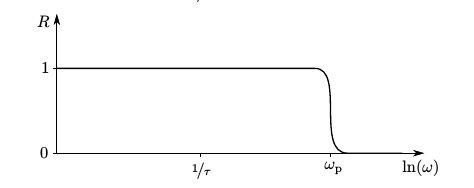
\includegraphics[scale=0.8]{Bilder/drude_reflektivitat.png} 
\caption{Reflektivität nach dem Drude Modell}
\label{fig:drude}
\end{figure}

Für kleine Frequenzen ist die Reflektivität nahezu 1, bei der Plasmafrequenz sinkt sie steil auf 0 ab.
Eine quantenmechanische Beschreibung kommt mit verschiedenen Annahmen zum gleichen funktionellen Ergebnis. Deshalb wird der Einfachheit halber, gern das Drude Modell angewendet.

Im Versuch werden Fabry-Perot-Filter (Abbildung \ref{fig:fabry}) hergestellt aus einer Schicht aus Dielektrikum versehen mit zwei hochreflektierenden dünnen Metallschichten.
Durch die Reflexschichten wird das Licht viele Male reflektiert. Dadurch entstehen Interferenzeffekte.

\begin{figure}[H]
\centering
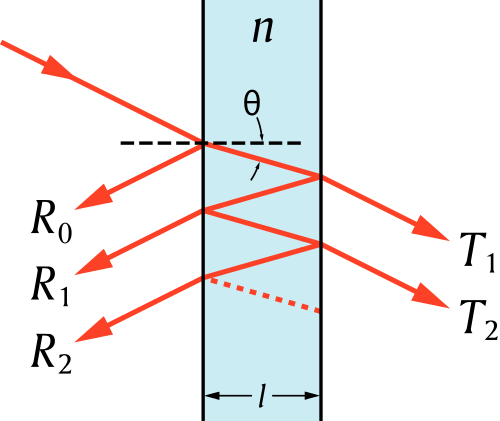
\includegraphics[scale=0.3]{Bilder/fabry_perot.png} 
\caption{Fabry-Perot-Filter}
\label{fig:fabry}
\end{figure}

Konstruktive Interferenz ergibt sich für:

\begin{gather}
\Delta \phi = \frac{4 \pi}{\lambda} n l \cos(\beta )- 2 \delta  \overset{!}{=} 2 \pi m \, \, \, \, \,  \, \, , m \,\epsilon \, \mathbb{N}_0. \\ 
\begin{matrix}
   \text{mit:} &&\\
   \phi & \text{--} & \text{Phasendifferenz} \\
   \lambda & \text{--} & \text{Wellenlänge des Lichts} \\
   n & \text{--} & \text{Brechungsindex des Dielektrikums} \\
   l & \text{--} & \text{Dicke des Dielektrikums} \\
   \beta & \text{--} & \text{Einfallswinkel des Lichts} \\
   \delta & \text{--} & \text{Phasensprung am Metall} \\
\end{matrix}\notag
\end{gather}

\section{Versuchsaufbau und Versuchsdurchführung}

Der Versuch wird durchgeführt mit einer Aufdampfanlage der Firma Edwards.

Zunächst wird die Vorpumpe eingeschaltet, die 15 min warmläuft. 
In dieser Zeit wird der Versuchsapparat gesäubert 
(mit einem Staubsauger und Isopropylalkohol Flies).
Dann wird ein Glasplättchen in den Probenhalter eingesetzt. Auf dieses Plättchen werden im Versuch die Schichten aufgedampft. Der Shutter wird so platziert, dass er das Glasplättchen blockiert, die Schwingquarzwaage aber frei ist.
Das Plattenventil ist geschlossen, muss allerdings freigängig sein, ist es dieses nicht, schaltet man die Turbopumpe kurz an, und wieder aus, und achtet darauf, dass Stickstoff für die Belüftung der Pumpe bereitsteht.
Es wird eine Folie im Rezipienten eingebracht, damit weniger Material auf die Glasglocke aufdampft. Der Rezipient wird geschlossen, und das Plattenventil wieder geöffnet. Das Handventil zur Vorpumpe wird geöffnet. Nachdem die Vorpumpe einen Druck von 10 nbar erreicht hat,wird die Turbopumpe dazugeschaltet. Wenn die Turbopumpe einen Druck in der Größenordnung $10^{-5}$ erreicht hat, wird der Bedampfprozess gestartet.

Es werden folgende Präparate hergestellt.
\begin{enumerate}[itemsep=0pt] 
\item 200 nm Silber
\item 20 nm Silber - 500 nm Kryolith
\item 20 nm Silber - 151 nm Kryolith - 20 nm Silber
\item 20 nm Silber - 500 nm Kryolith - 20 nm Silber
\end{enumerate}
Bei einem Präparat wird vor dem Bedampfen mit Kryolith eine Reflexions- und Transmissionsmessung für die 20 nm dicke Silberschicht durchgeführt.

Beim Aufdampfen auf das Substrat sollte die Aufdampfrate zwischen 10 und 20 $\buildrel _{\circ} \over {\mathrm{A}}$/s liegen.

Die Schwingquarzwaage muss auf die Dichte des Materials eingestellt werden.

Nach dem Bedampfen muss darauf geachtet werden, dass der Ballon an der Stickstoffkanne dauerhaft aufgeblasen ist. Die Turbopumpe wird abgeschaltet, das Handventil zur Vorpumpe geschlossen, und das Plattenventil geschlossen. Der Rezipient wird belüftet.
Die Turbopumpe braucht eine Weile, um herunterzufahren.
Der Rezipient wird erneut gereinigt.

Für die Messung der optischen Eigenschaften steht ein Aufbau für Reflexions- und Transmissionsmessung bereit.

\newpage

\section{Auswertung}

\subsection{Metallschichten einer Dicke von 200 und 20 nm}

Zunächst werden auf zwei Glasplättchen 200 nm bzw. 20 nm Silber aufgedampft. Die Proben werden auf ihre spektralen Eigenschaften im Bereich einer Wellenlänge von 300 bis 1000 nm untersucht.
Die gemessene Intensitäten für Transmission und Reflexion sind in Abbildung \ref{fig:spiegel} bzw. \ref{fig:m_20nm} dargestellt.

Das verwendete Spektrometer misst in einem Bereich von 300 bis 1000 nm Wellenlänge. Besonders im unteren Rand des Bereiches, und auch am oberen, misst das Spektrometer sehr groß schwankende Werte, und Intensitäten weit über 100 \%.
Es wird nur ein angepasster Wertebereich geplottet, da sonst aus den Abbildungen kein Gehalt ausgelesen werden kann.
\begin{figure}[H]
\centering
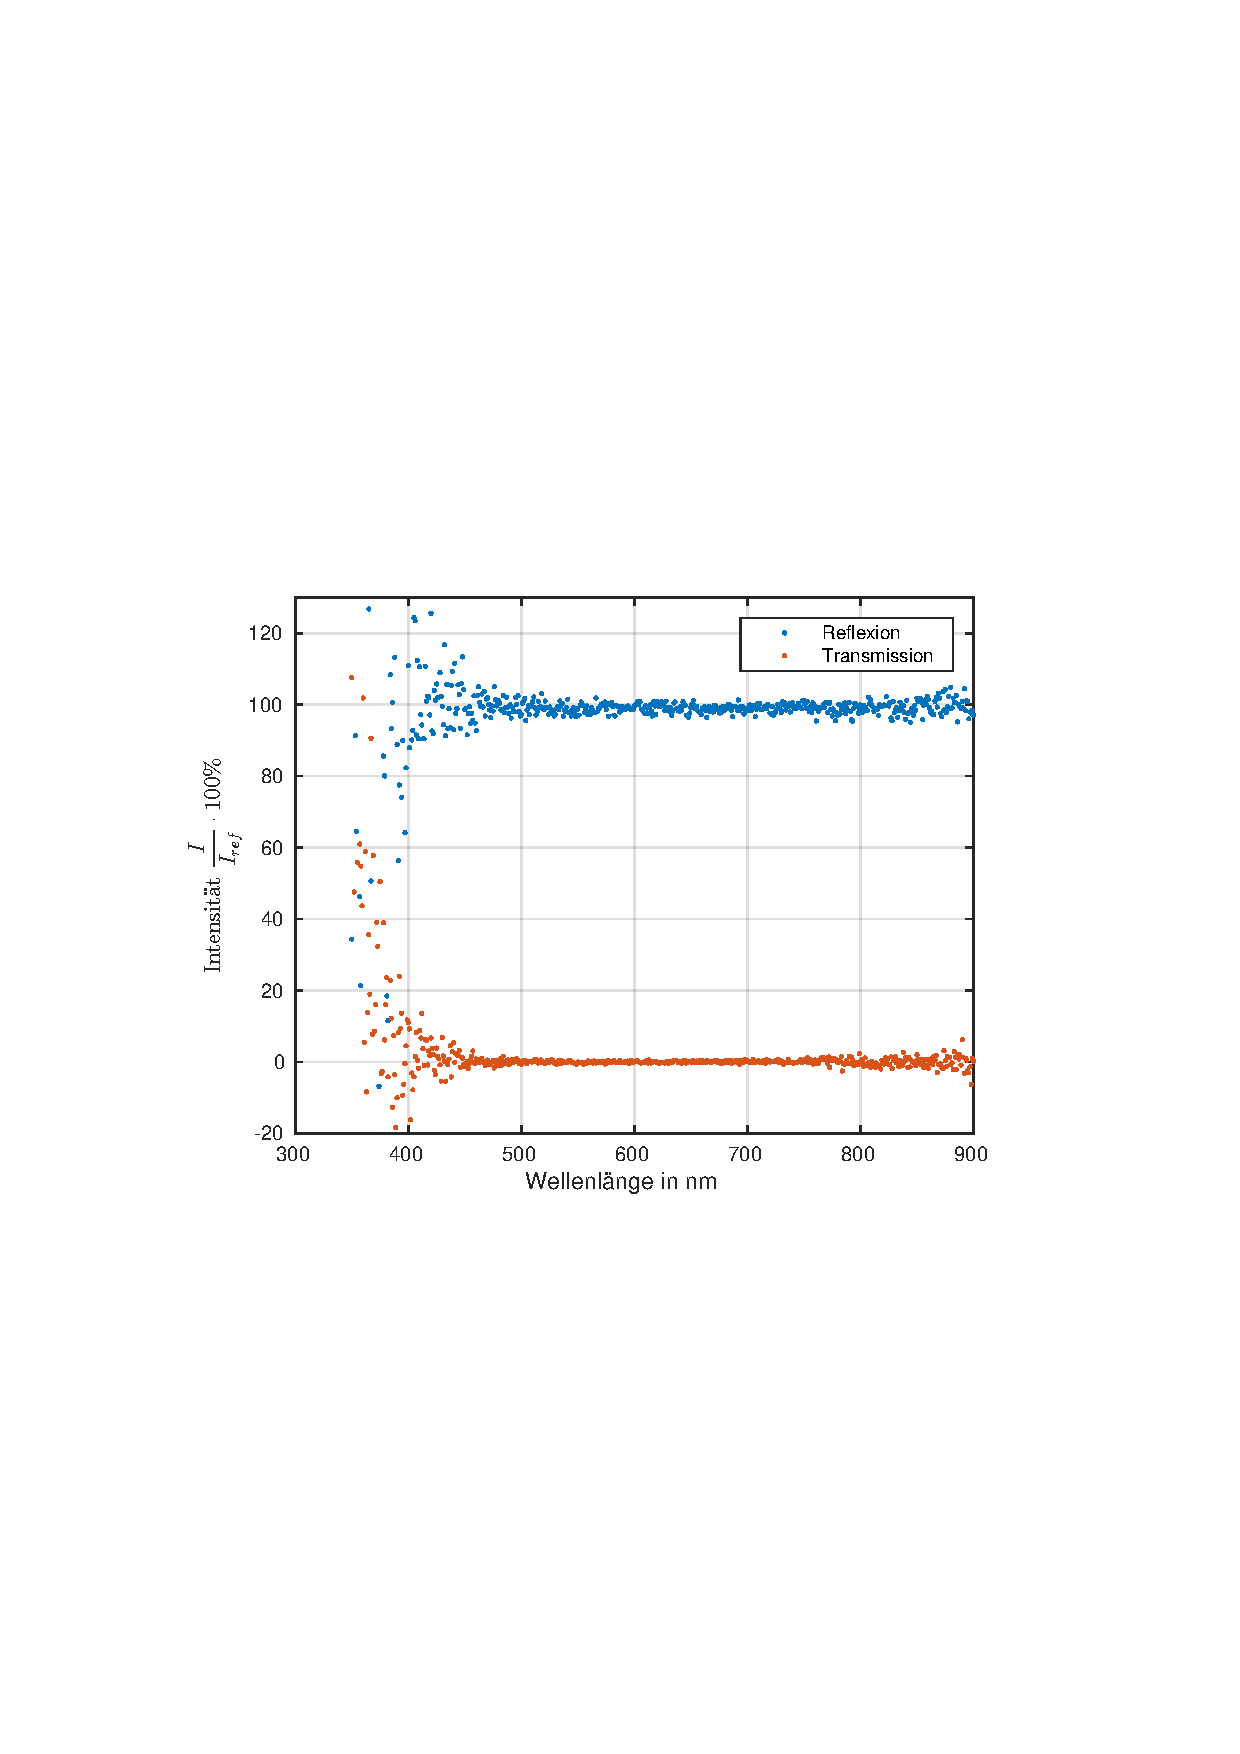
\includegraphics[trim = 1.1in 3.7in 1.1in 3.9in, clip, scale=1]{../Messdaten/Plots/spiegel_200.pdf} 
\caption{Transmission und Reflexion an einer 200 nm dicken Silberschicht.}
\label{fig:spiegel}
\end{figure}
Die 200 nm dicke Silberschicht verhält sich wie ein Spiegel. Die Reflexion im gemessenen Bereich beträgt annähernd 100 \%, die Transmission 0 \%. Es wird also in guter Näherung nichts absorbiert.

Diese Probe wird wegen dieser Eigenschaften in den weiteren Reflexionsmessungen als Referenzprobe verwendet. Für kleine Wellenlängen stellt sie jedoch keine ideale Referenzprobe dar.

Etwas anders sehen die Messungen der nur 20 nm dicken Silberschicht aus. In Abbildung \ref{fig:m_20nm} sind die Messdaten geplottet, sowie eine Simulation der Transmission.
Die Reflexion liegt bei etwa 90 \% im oberen Messbereich und fällt hin zu kleineren Wellenlängen leicht ab auf etwa 85 \%.
Eine Schichtdicke von 20 nm ist also so dünn, dass Licht hindurchscheint. Hält man die Probe gegen das Licht, sieht man bereits mit blossem Auge, dass sie teils durchlässig ist.
Mit der Software \textit{WASF} wird eine Simulation des Schichtsystems durchgeführt.
In der Simulation ist die Transmission höher als in der Messung, der Verlauf an sich stimmt jedoch überein.
Vermutlich ist die aufgedampfte Schicht dünner als 20 nm.

\begin{figure}[H]
\centering
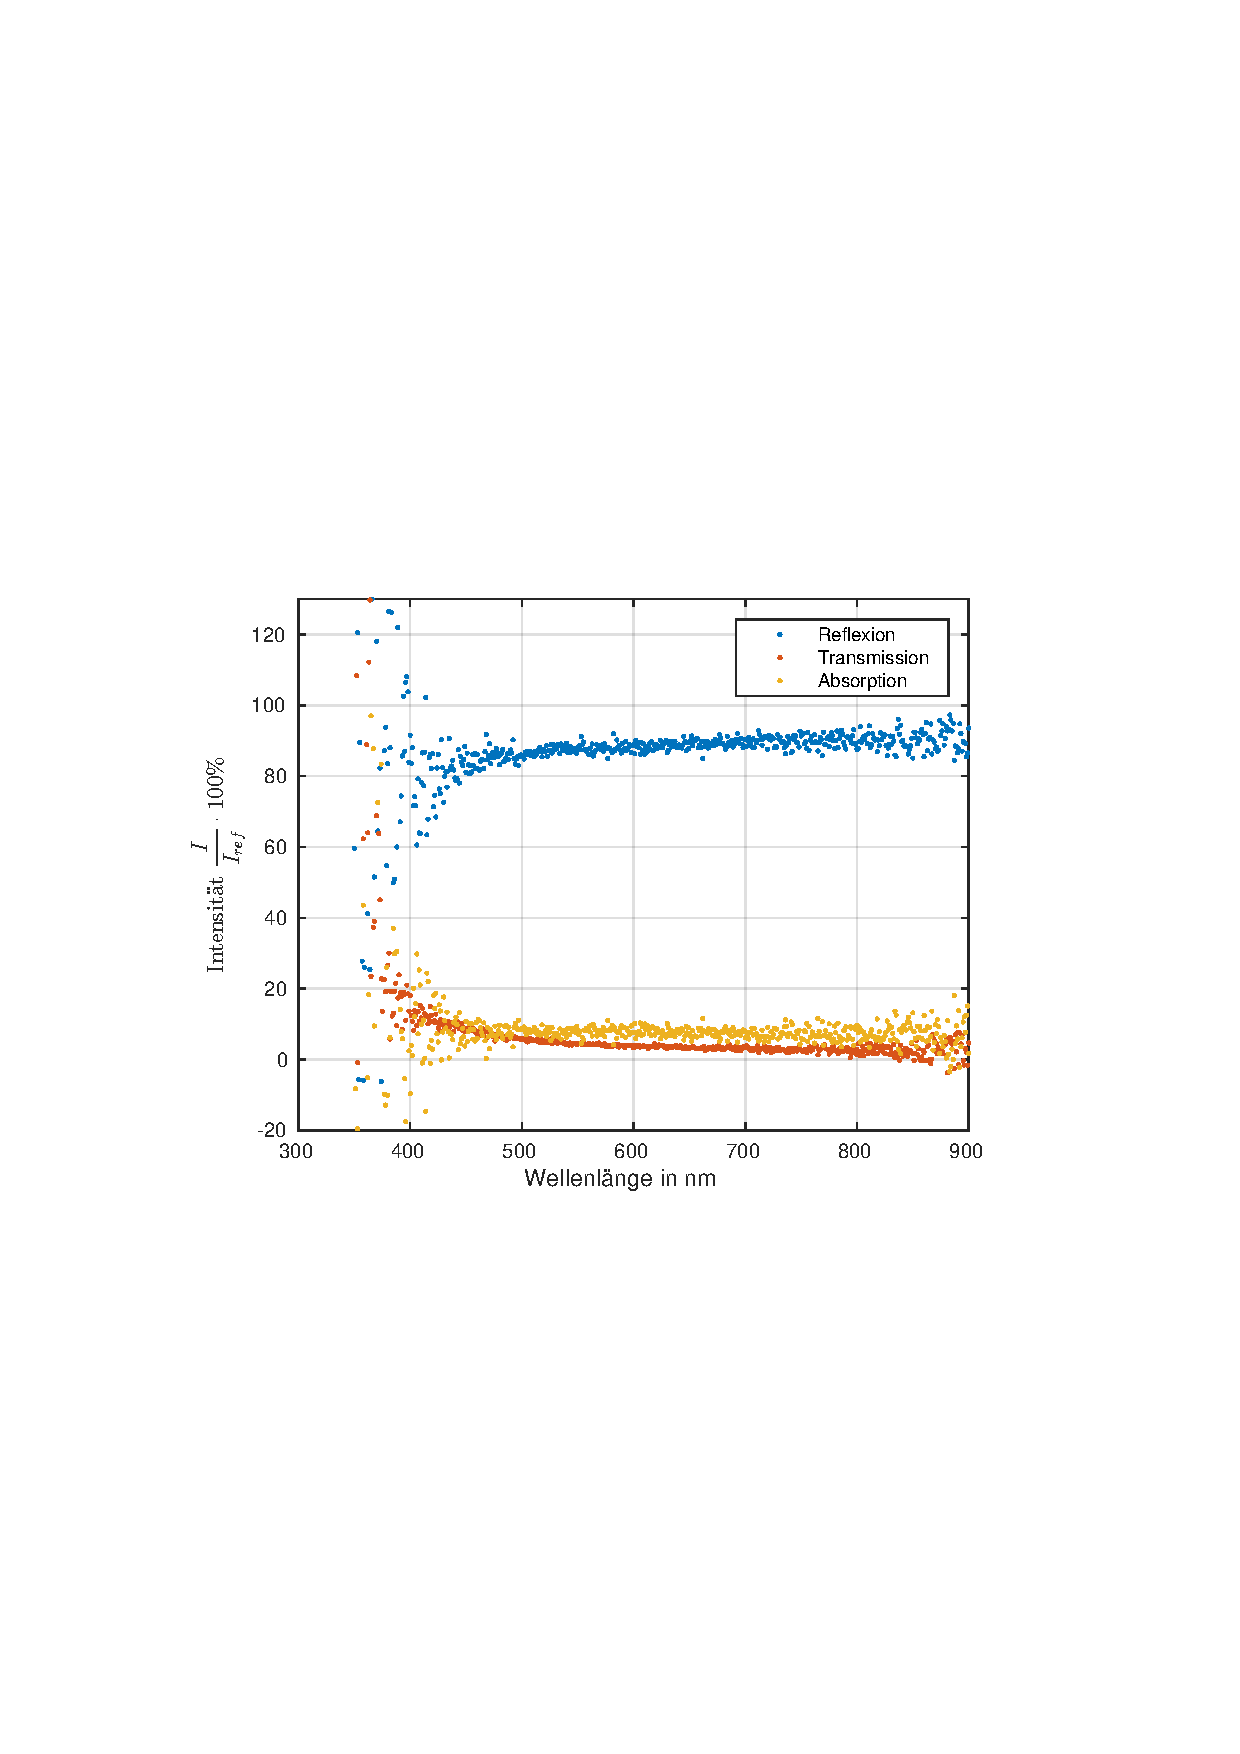
\includegraphics[trim = 1.1in 3.7in 1.1in 3.9in, clip, scale=1]{../Messdaten/Plots/m_20nm.pdf} 
\caption{gemessene Intensitäten der Transmission und Reflexion an einer 20 nm dicken Silberschicht. Die Absorption wurde aus den Daten berechnet. Außerdem wurde die Transmission zum Vergleich mit der Software \textit{WASF} simuliert.}
\label{fig:m_20nm}
\end{figure}

Nach dem Drude-Modell liegt die Reflektivität eines Metalls für kleine Frequenzen bei annähernd 100 \%, und fällt mit steigender Frequenz bei der Plasmafrequenz steil auf 0 \% ab. Die Plasmakante von Silber liegt bei einer Wellenlänge von ca. 322 nm. [1] 

Leider funktioniert das vorhandene Spektrometer im Bereich nur zuverlässig in einem Bereich von 400 nm bis 900 nm, weshalb die Plasmakante nicht beobachtet werden kann. Ein leichter Abfall der Reflaktivität ab 450 nm zu kleineren Frequenzen hin, ist jedoch zu erkennen.

\newpage

\subsection{Zweischichtsystem aus 20 nm Metall und 500 nm Dielektrikum}

Es wird eine Probe hergestellt aus 20 nm Silber und 500 nm Kryolith.
Die gemessenen optischen Eigenschaften sind in Abbildung \ref{fig:md_500} dargestellt.

\begin{figure}[H]
\centering
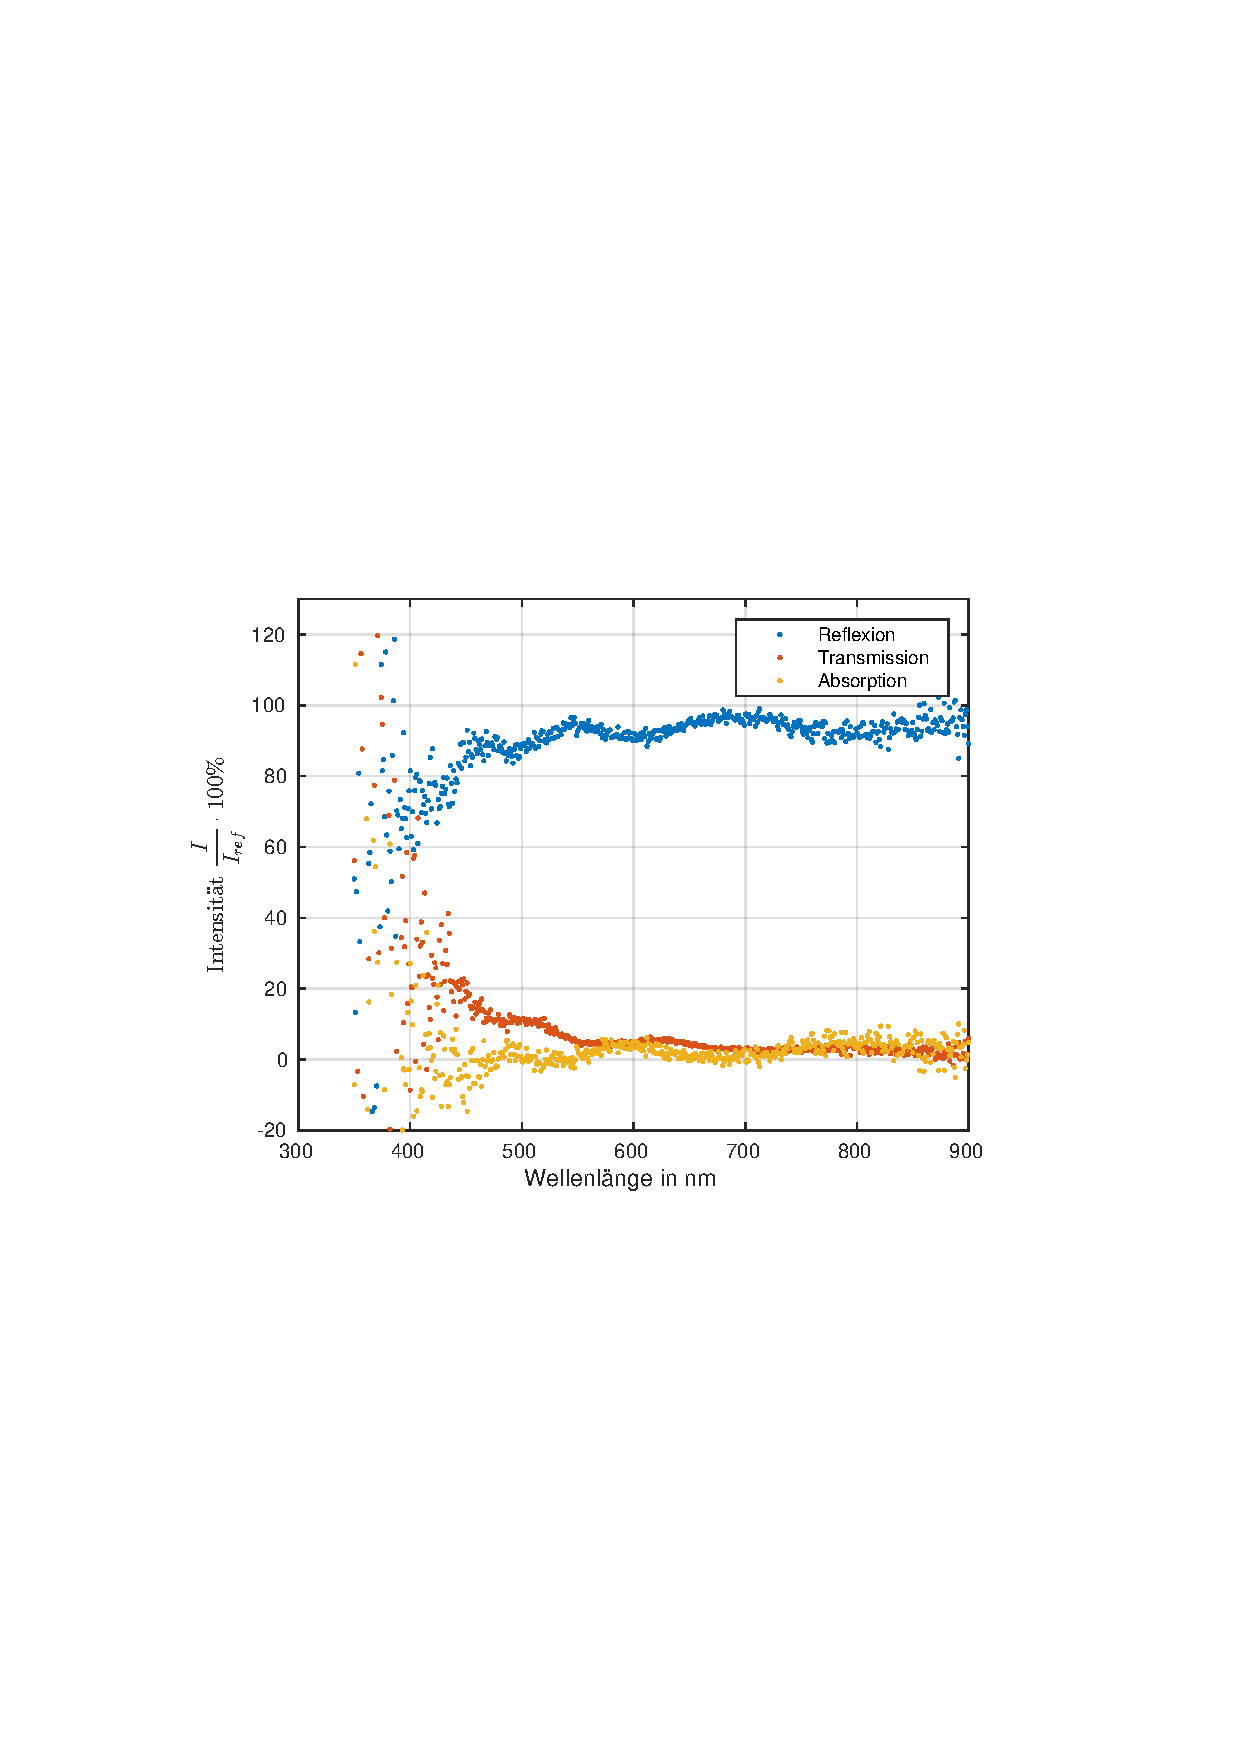
\includegraphics[trim = 1.1in 3.7in 1.1in 3.9in, clip, scale=1]{../Messdaten/Plots/md.pdf} \caption{gemessene Intensitäten der Transmission und Reflexion an einem Zweischichtsystem aus 20 nm Metall und 500 nm Dielektrikum. Die Absorption wurde aus den Daten berechnet.}
\label{fig:md_500}
\end{figure}

Die Messungen zeigen leicht frequenzabhängiges Verhalten, die Reflektivität ist jedoch im gesamten gemessenen Bereich hoch, zwischen 60 \% und 100 \%.
Zu kleineren Welenlängen fällt die Reflektivität dabei ab.

Mit WASF wird auch zu diesem Schichtsystem eine Simulation gemacht (Abbildung \ref{fig:md_500_sim}).
Die Messung weicht von der Simulation stark ab. Vielleicht war die Messung der Probe fehlerhaft.
In Kapitel 3.4 wird die Dicke der aufgedampften Kryolith-Schicht bestimmt, da die Simulation an diese Messdaten besser angepasst werden kann.

\begin{figure}[H]
\centering
\includegraphics[trim = 1.1in 3.7in 1.1in 3.9in, clip, scale=1]{../Messdaten/Plots/simulation_m20_d500.pdf} 
\caption{simulierte Intensität der Transmission an einem Zweischichtsystem aus 20 nm Metall und 500 nm Dielektrikum mit dem Programm \textit{WASF}.}
\label{fig:md_500_sim}
\end{figure}

Ein sinnvolles Filter stellt die Probe nicht dar. Die Eigenschaften ändern sich allerdings drastisch, wenn man auf der anderen Seite der Kryolithschicht eine zweite Silberschicht hinzufügt, was im nächsten Versuchsteil untersucht wird.

\newpage

\subsection{Filter für 520 nm}

Es wird ein Interferenzfilter hergestellt für eine Wellenlänge von 520 nm.
Die dafür benötigte Schichtdicke d des Dielektrikums, bei senkrechtem Lichteinfall, und für das Maximum 0. Ordnung ergibt sich aus der Formel:

\begin{gather}
d = \frac{\delta \lambda}{2 \pi n}\\
\begin{matrix}
   \text{mit:} &&\\
   \delta \lambda & \text{--} & \text{Phasensprung an Silber bei 520 nm, }\delta \lambda \approx 140^\circ \\
   n & \text{--} & \text{Brechungsindex des Dielektrikums (Kryolith), } n \approx 1,338 \\
\end{matrix}\notag
\end{gather}

Daraus ergibt sich, dass 151 nm Kryolith aufgedampft werden.
Die spektralen Eigenschaften des Filters sind in Abbildung \ref{fig:mdm_151} dargestellt.

\begin{figure}[h]
\centering
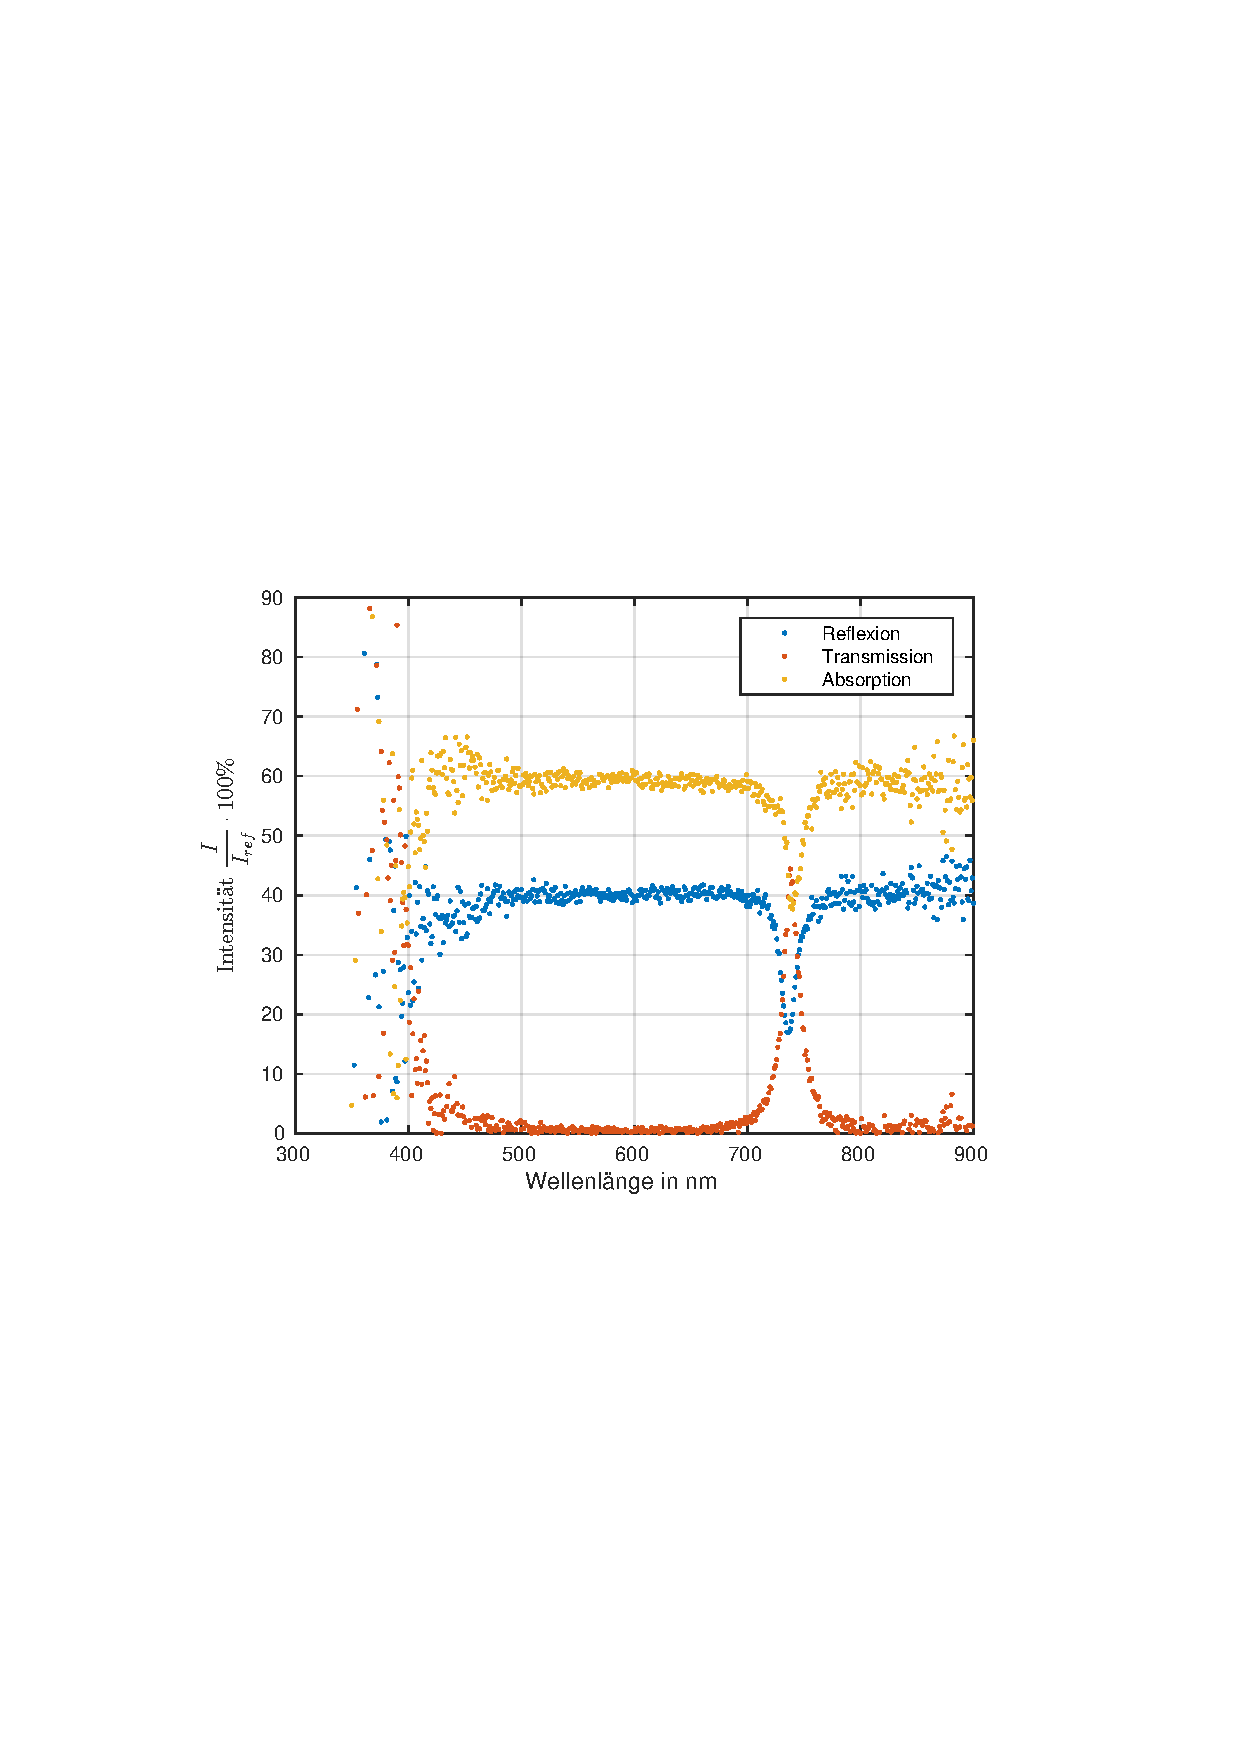
\includegraphics[trim = 1.1in 3.7in 1.1in 3.9in, clip, scale=1]{../Messdaten/Plots/filter_151_zoom.pdf} 
\caption{gemessene Intensitäten der Transmission und Reflexion an einem Filter aus einer etwa 151 nm dicken Kryolithschicht versehen mit hochreflektierenden Schichten. Die Absorption wurde aus den Daten berechnet. Außerdem wurde die Transmission, bei angepasster Schichtdicke, zum Vergleich mit der Software \textit{WASF} simuliert.}
\label{fig:mdm_151}
\end{figure}

\newpage

Die Abbildung zeigt, dass zwar im untersuchten Spektralbereich ein Filter hergestellt wurde, jedoch wurde die gewünschte Wellenlänge von 520 nm grob verfehlt. 
Aus den Messdaten ergibt sich, dass tatsächlich ein Filter für 737 nm hergestellt wurde. Es wurde also statt eines Filters für grünes Licht, eines für rotes hergestellt.

Der Peak ist relativ scharf, mit einer Halbwertsbreite von 16 nm. Die Güte des Filters hängt maßgeblich von der Reflektivität der Metallschichten ab. Je höher die Reflektivität, desto schärfer sind die Peaks.
Der Quality-Faktor ist definiert als:
\begin{equation}
Q=\frac{\nu_0}{\Delta \nu} = \dfrac{\dfrac{1}{\lambda_0}}{\dfrac{1}{\lambda_{-}}-\dfrac{1}{\lambda_{+}}}
\end{equation}
Dabei ist $\nu_0$ bzw. $\lambda_0$ die Frequenz bzw. Wellenlänge des Transmissionsmaximum, $\Delta \nu$ die volle Halbwertsbreite, und  $\lambda_{-}$ und $\lambda_{+}$ die Werte, bei denen der Peak auf die Hälfte abgefallen ist.Aus den Messungen ergibt sich für das Filter ein Q-Faktor von $Q=46$.
Im Vergleich zur Simulation hat das Filter eine höhere Güte, was vermutlich durch die abweichende Dicke der Silberschichten bedingt ist.

Die tatsächlich aufgedampfte Schichtdicke lässt sich aus Formel 4 oder durch Verändern der Parameter der Simulationssoftware \textit{WASF}.
Aus der Berechnung mit Formel 4 folgt eine Schichtdicke von 230 nm. (Dabei wird die tatsächliche Wellenlänge von 737 nm und ein Phasensprung von $150^\circ$ eingesetzt).
Mit \textit{WASF} wird zunächst das Schichtsystem mit 20-151-20 simuliert, und dann die Schichtdicke des Kryolith so angepasst, dass ein den Messdaten ähnliches Bild entsteht. Mit dieser Methode ergibt sich eine Schichtdicke von 250 nm.

Die Reflektivität bei den nicht durchgelassenen Frequenzen beträgt nur 40 \%. Somit hat man eine hohe Absorption (und Streuung) von 60 \%. Vielleicht wurde eine fehlerhafte Referenzmessung durchgeführt.


\subsection{Interferenzfilter mit 500 nm Dielektrikum}

Die letzte hergestellte Probe ist ein Schichtsystem aus 20 nm Silber - 500 nm Kryolith - 20 nm Silber.
Die optischen Eigenschaften der Probe sind in Abbildung \ref{fig:mdm_500} dargestellt, zusammen mit einer Simulation des Systems mit angepasster Kryolith-Dicke.

\begin{figure}[h]
\centering
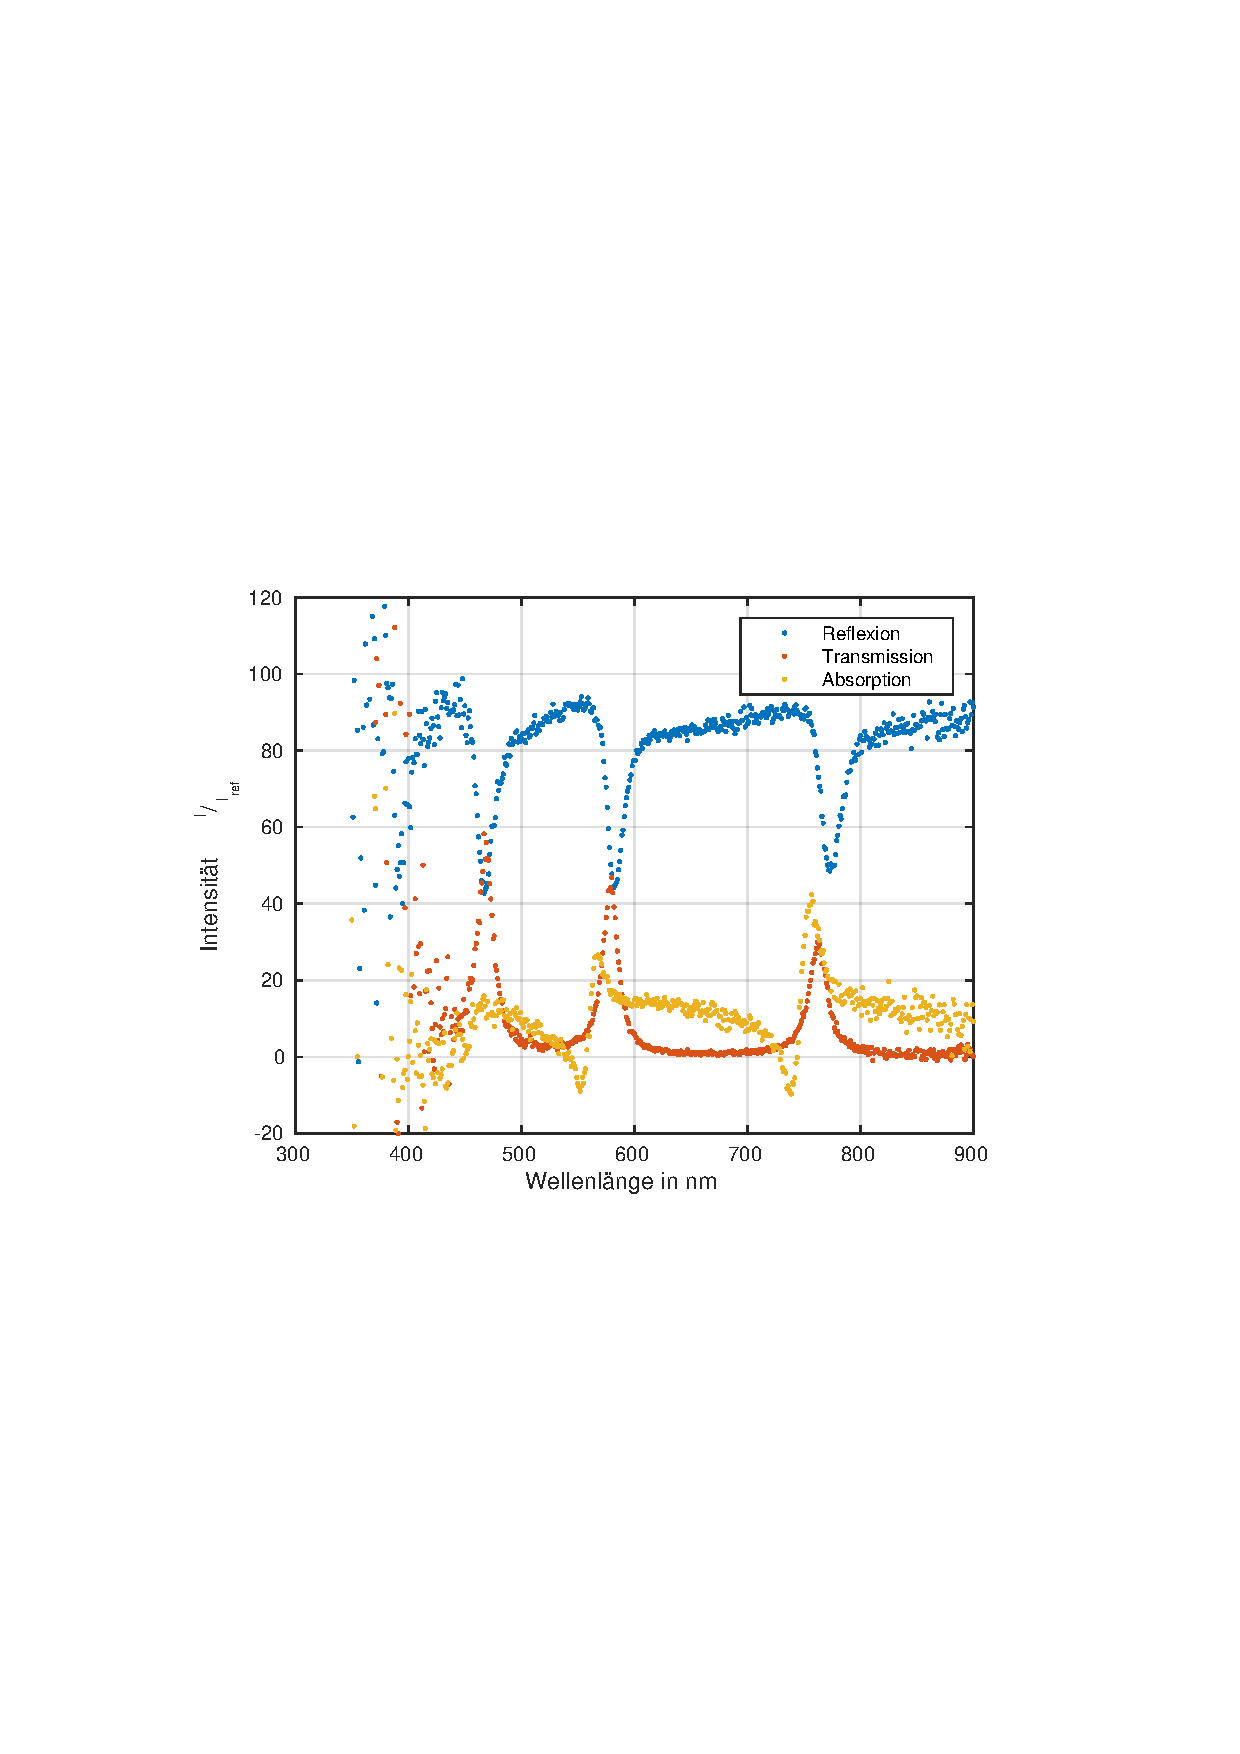
\includegraphics[trim = 1.1in 3.7in 1.1in 3.9in, clip, scale=1]{../Messdaten/Plots/mdm_500.pdf} 
\caption{gemessene Intensitäten der Transmission und Reflexion an einem Filter aus einer etwa 500 nm dicken Kryolithschicht versehen mit hochreflektierenden Schichten. Die Absorption wurde aus den Daten berechnet. Außerdem wurde die Transmission, bei angepasster Schichtdicke, zum Vergleich mit der Software \textit{WASF} simuliert.}
\label{fig:mdm_500}
\end{figure}

Im untersuchten Spektralbereich liegen drei Beugungsmaxima, bei 467 nm, 581 nm und 762 nm.
Die Reflexion außerhalb der durchgelassenen Frquenzen ist hier wieder höher, im Bereich von 90 \%.
Mit dem Programm \textit{WASF} wird das Schichtsystem simuliert.
Dabei wird mit die Dicke der Kryolith-Schicht zunächst auf 500 nm gestellt, und dann variiert, bis die Simulation den Messdaten entspricht. Die so bestimmte Schichtdicke beträgt 910 nm.

Ein Vergleich mit dem gesamten simulierten Spektrum zeigt, dass im untersuchten Spektralbereich die Beugungsmaxima zweiter, dritter, und vierter Ordnung liegen.

\section{Fehlerbetrachtung}

Die größten Fehlerquellen in diesen Versuch sind Verunreinigungen im Rezipienten und eine unstetige Aufdampfrate. Weiter sollte darauf geachtet werden, 
dass die Turbopumpe in der Größenordnung von $10^{-5}$\,mbar liegt. In unserem Versuch hat dies die Turbopumpe selbst nach längerem warten nicht mehr erreicht. Über den genauen Grund sind wir uns nicht im klaren. Wir durften aber, da dies der letzte Aufdampfprozess war, dennoch schon bei $4\cdot 10^{-4}$\,mbar aufdampfen. 
Hier hatten wir eine besonders unstetige Aufdampfrate, die kurzzeitig sogar 50\,$\buildrel _{\circ} \over {\mathrm{A}}$/s erreichte. 
Eine zu hohe Aufdampfrate kann dazu führen, dass man den gewollten homogenen Schichtwachstum (Franck der Merve-Wachstum) nicht bekommt, sondern einen inhomogenen Schichtwachstum. Bei der Transmissions- und Reflexionsmessung ist zudem zu beachten, dass die Referenzmessung sauber gemessen werden.

\newpage

\section{Zusammenfassung}

Im ersten Versuchsteil ergab sich bei uns, dass das Glasplättchen, welches mit 200\,nm Silber aufgedampft wurde, als Spiegel fungiert. Das mit 20\,nm Silber aufgedampfte jedoch nicht. In unseren Messungen lag die Reflexion bei etwa 90\%.

Bei der Betrachtung des Zweischichtsystem aus 20\,nm Metall und 500\,nm Kryolith ist aus unseren Messungen ein Wellenlängenfiltereffekt abzulesen, da bestimmte Wellenlängen stärker transmittiert werden.

Durch hinzufügen einer weiteren Silberschicht, sodass die Kryolithschicht auf beiden Seiten eine Silberschicht aufweist, ist ein deutlich besserer Wellenlängenfilter gebaut worden. In unserem Versuch filtern wir rotes Licht mit etwa der Wellenlänge 737\,nm am Effektivsten, was laut \textit{WASF} auf eine Schichtdicke von nur 136\,nm Kryolith schließen lässt. 

Zum Schluss haben wir das Schichtsystem aus 20\,nm Silber - 500\,nm Kryolith - 20\,nm Silber, indem wir mit unseren Messungen die Interferenzfiltereigenschaften gut beobachten können. Jedoch haben wir auch hier laut \textit{WASF} eventuell zu wenig aufgedampft. 

\renewcommand{\refname}{\textbf{Literaturverzeichnis}}
\begin{thebibliography}{xxxxxxxxxxxxxxx}

 		  \bibitem[1]{1}		\glqq E. Hecht, Optik\grqq~3., vollst. überarb. Aufl., Oldenbourg Verlag, München 2001, Gebunden 
ISBN 3-486-24917-7
		 
\end{thebibliography}

\end{document}